\documentclass{article}
\pdfpagewidth=8.5in
\pdfpageheight=11in
\usepackage{ijcai26}
\usepackage{times}
\usepackage{url}
\usepackage[hidelinks]{hyperref}
\usepackage[utf8]{inputenc}
\usepackage[small]{caption}
\usepackage{graphicx}
\usepackage{amsmath}
\usepackage{amsthm}
\usepackage{booktabs}
\urlstyle{same}

\title{Cost-Sensitive Triage of Supplier Bank-Change Requests:\\A One-Step Bayesian Agent on 40 Simulated Cases\thanks{Course preprint. Not submitted to IJCAI. All cases are simulated.}}
\author{
    Student Project
    \affiliations
    AI-Native Engineering, Course Project
}

\begin{document}
\maketitle

\begin{abstract}
A supplier bank-change request arrives with its hidden state unknown: the supplier's
genuine intent or fraud from a compromised channel. We build a POMDP-inspired one-step
agent that maintains a Bayesian belief over \{Genuine, Fraud\} and selects among
APPROVE, VERIFY (out-of-band callback), and ESCALATE (human controller) by expected
cost. Evaluated blind on 40 simulated labeled cases (32 genuine, 8 fraud) against a
rule-checklist agent, an email-authentication baseline, and two reference ceilings, the
Bayesian policy catches all 8 frauds at \$4,200 total cost versus \$143,374 for the
baseline. Accuracy alone (0.85 vs.\ 0.80) hides a \$139k cost gap. Likelihoods and
costs are stated assumptions with a sensitivity procedure, not measured facts.
\end{abstract}

\section{Introduction}
The agent reads a supplier bank-change request. It must approve, verify via a second
channel, or escalate to a human, because it cannot yet tell whether the request
reflects the supplier's genuine intent. Email authentication passes even on a fully
compromised mailbox, so it cannot carry the decision \cite{sysadmin-thread}. A wrong
approval loses the wire irreversibly; a wrong check costs only callback labor and
delay. The contribution is a tested, cost-sensitive triage policy: full predictions,
multi-metric scoring beyond accuracy, six named failure modes, and repeat
instructions, all on one fixed 40-case simulation.

\section{Related Work and User Discussions}
Practitioner discussions shaped every design choice. Operators report that
verify-everything policies collapse under volume into rubber-stamping, and that calm,
long-game fraud with no urgency signal is where losses concentrate
\cite{aiagents-thread}. Bank-verification APIs are judged a supplement that does not
replace callback verification for bank-change events \cite{fintechdev-thread}.
Practitioners verify changes by voice on a pre-known number, confirm by email to a
known address, and inherit \$5--10k counter-signature materiality thresholds
\cite{accounting-thread}. Authentication passes clean on mailbox compromise, leaving
behavioral signals and procedural voice verification as the closing control
\cite{sysadmin-thread}. These findings set the evidence set, the callback-first
action, and the weak weight on email authentication.

\section{Agent Design}
Input: one request record (callback status, first-time flag, urgency, reply-to drift,
lookalike domain, tone deviation, email-auth status, amount). Hidden state:
$S \in \{\mathrm{Genuine}, \mathrm{Fraud}\}$. Belief: $P(S\mid\mathrm{evidence})$.
Actions: APPROVE (pay), VERIFY (out-of-band callback, \$150 assumed), ESCALATE
(controller hold and review, \$500 assumed). Cost: approving fraud loses the full
amount; approving genuine costs \$0; checks cost their flat fees. Policy: the
expected-cost rule of Section~5. Feedback: the callback outcome or controller verdict
becomes new evidence for a belief update. The built-in human function is sending
high-cost uncertain decisions to a human: posteriors at or above 0.65 escalate
directly. This is the smallest testable version: a Naive Bayes update plus threshold
code, no sequential planner.

\section{Probability Model and Decision Rule}
With prior $P(F)=0.10$ (assumed base rate, not fitted to test labels) and a priori
likelihoods $P(e_i\mid S)$ set from discussion direction, the posterior is
\begin{equation}
P(F\mid e_{1:k}) =
\frac{P(F)\prod_i P(e_i\mid F)}
{P(F)\prod_i P(e_i\mid F)+P(G)\prod_i P(e_i\mid G)},
\label{eq:post}
\end{equation}
with $P(G\mid e_{1:k})=1-P(F\mid e_{1:k})$, so beliefs always sum to 100\%.
Expected costs at posterior $p$ and amount $A$ are
\begin{equation}
\begin{aligned}
E[C\mid\mathrm{APPROVE}] &= p\cdot A,\\
E[C\mid\mathrm{VERIFY}] &= 150,\\
E[C\mid\mathrm{ESCALATE}] &= 500.
\end{aligned}
\label{eq:cost}
\end{equation}
Decision rule: ESCALATE if $p\ge 0.65$; APPROVE if $p\cdot A<150$ and $p<0.35$;
otherwise VERIFY; high-value guard escalates when $A>20{,}000$ and $p\ge 0.25$.
Example (case C030, checked): likelihood products give $p=0.3613$ via
Eq.~\ref{eq:post}; Eq.~\ref{eq:cost} gives $\$2{,}768$ vs.\ $\$150$ vs.\ $\$500$,
hence VERIFY; a later failed callback updates the belief to $0.9314$ and the action
to ESCALATE. The true label is stripped before every policy call and used only for
scoring.

\section{Test Method}
One fixed simulation of 40 labeled cases (32 genuine, 8 fraud) stored in
\texttt{data/\allowbreak{}supplier\_\allowbreak{}bank\_\allowbreak{}change\_\allowbreak{}simulated\_\allowbreak{}dataset.xlsx}
\cite{bankchange-data}. Two agent policies (Bayesian cost-sensitive; deterministic
red-flag checklist with zero weight on email authentication) plus an email-auth
baseline (approve iff authentication passes) and two reference ceilings
(always-approve, always-verify). Metrics beyond accuracy: confusion matrix,
precision, recall, false-positive and false-negative counts, human-review rate,
decision cost, and binned calibration (ECE). Every case$\times$policy prediction is
saved in \texttt{results/\allowbreak{}predictions.csv} (200 rows). The manuscript is formatted
with the official IJCAI-ECAI-2026 author kit \cite{ijcai-kit}.

\section{Results}
Table~\ref{tab:res} and Figure~\ref{fig:cost} summarize the blinded run.

\begin{table}[t]
\centering
\caption{Blinded results on 40 simulated cases.}
\label{tab:res}
{\footnotesize\setlength{\tabcolsep}{3pt}
\begin{tabular}{lrrrrr}
\toprule
Policy & TP/FP/TN/FN & Prec & Rec & Rev. & Cost \$ \\
\midrule
Bayesian & 8/6/26/0 & 0.571 & 1.000 & 0.350 & 4,200 \\
Checklist & 8/13/19/0 & 0.381 & 1.000 & 0.525 & 6,300 \\
SPF baseline & 1/1/31/7 & 0.500 & 0.125 & 0.050 & 143,374 \\
Always approve & 0/0/32/8 & 0.000 & 0.000 & 0.000 & 150,736 \\
Always verify & 8/32/0/0 & 0.200 & 1.000 & 1.000 & 6,000 \\
\bottomrule
\end{tabular}}
\end{table}

\begin{figure}[t]
\centering
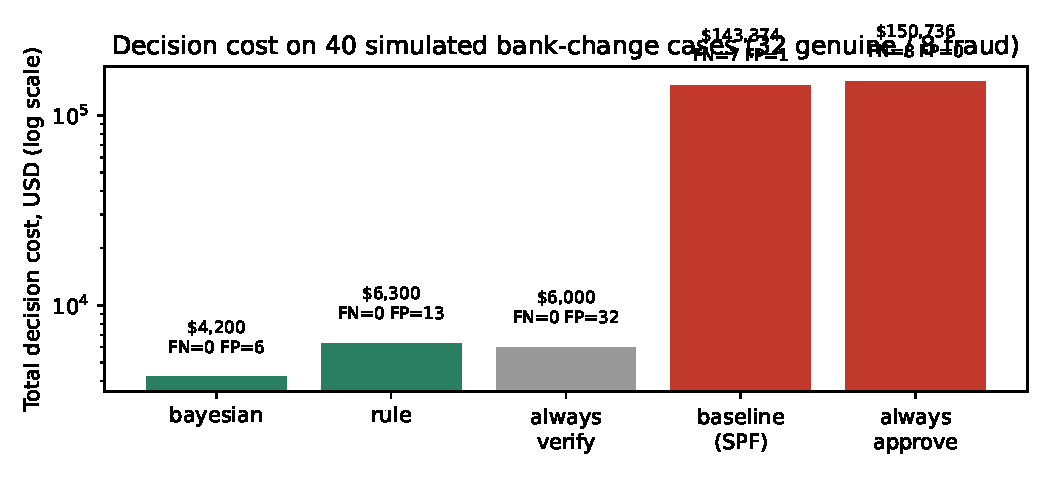
\includegraphics[width=\columnwidth]{figures/costs.pdf}
\caption{Total decision cost per policy (log scale), annotated with false negatives
(FN) and false positives (FP). The Bayesian policy pays bounded check costs to avoid
all wire losses.}
\label{fig:cost}
\end{figure}

Both agents reach recall 1.000 with zero fraud loss; the baseline misses 7 of 8
frauds (recall 0.125) because authentication passes on compromise. Calibration ECE is
0.038 for the Bayesian policy (bins hold only 1--5 cases, so indicative only).
Every number in this section was re-verified against \texttt{results/\allowbreak{}metrics.json}.

\section{Failure Analysis}
Six examined errors, each named: Stolen-Callback Confirmation (fraud with a
``confirmed'' callback, \$54,729 at stake), Urgency-Free Sleeper (calm \$56,875
fraud), Repeat-Vendor Camouflage (fraud on a repeat vendor), Stale-Contact False
Alarm (genuine case with a failed callback, \$150 wasted), Legitimate-Urgency
Over-Triage (genuine first-time urgent change escalated), Benign Anomaly Coincidence
(genuine reply-to/tone drift). Highest cost: false APPROVE of fraud (false
negative), at \$3k--\$57k per miss versus \$150--\$500 per false alarm, because wires
are unrecoverable while delays are resolved by one callback --- a 20--380$\times$
asymmetry that justifies tuning for recall 1.000.

\section{Limitations, Ethics, and Human Control}
Simulated single 40-case split with no holdout; invented likelihoods under a false
independence assumption; hand-picked thresholds never swept; flat assumed costs with
zero recovery; small-sample calibration; 35--52\% review rates exceeding realistic
human capacity (rubber-stamp risk); trusted-but-unverified master-data numbers; and a
one-step rule rather than sequential planning. Ethics: all amounts are simulated and
must never be quoted as real fraud data. Human control is structural, not advisory:
uncertain high-cost cases escalate to a controller by policy, and number changes
require a separate authorization path.

\section{Conclusion and New Questions}
Cost-sensitive triage with hidden labels, multi-metric scoring, and named failures
turns a vague fraud problem into a testable policy choice. Open questions: sweeping
thresholds on a validation split; recovery-rate and capacity-budgeted costs; joint
likelihoods for correlated signals; and a live pilot with audit logging. Sensitivity
procedure: perturb each likelihood ratio $\pm50\%$ (halve the failed-callback ratio
$30\to15$) and confirm the zero-false-negative policy survives.

\section*{AI Use Statement}
Muse Spark (via OpenCode) drafted code, computed metrics, formatted LaTeX, and acted
as practitioner, probability, and preprint reviewer; 17 of 21 review comments were
accepted with reasons in \texttt{review-record.md}. All Reddit/X content is the
student's own questions and summaries; no AI conversation was fabricated; every test
reported was executed by \texttt{experiments/\allowbreak{}run\_experiment.py}.

\section*{Contribution}
Solo student work. Problem selection, public discussions, agent design, software
development, tests, citation checks, preprint sections, and PDF checks were all
performed by the student with AI assistance as stated above.

\bibliographystyle{named}
\bibliography{references}

\end{document}
